\def\dhtSensorWidth{2}
\def\dhtSensorHight{2.5}
\def\dhtBoardWidth{1.4}
\def\dhtBoardHeight{0.75}

\def\dhtBvlX{0.2}
\def\dhtBvlY{0.25}

\def\dhtPinHoleThickness{0.07}

\ctikzsubcircuitdef{spicdht} {
    p1, p2, p3%
} {
    coordinate (#1-origin)
    ++({\dhtSensorWidth/2},{(-\dhtSensorHight-\dhtBoardHeight)/2})
    node [inner sep = 0pt, anchor = center] {
        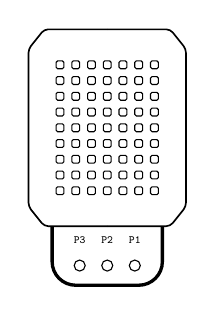
\begin{tikzpicture}
            %% markings
            \draw
            (0,0) coordinate (origin)
            (origin) ++({\dhtSensorWidth/2},0) coordinate (mid)
            ;
            \draw [semithick, rounded corners = 0.5mm]
            (mid) -- ++(-{\dhtSensorWidth/2+\dhtBvlX},0)
            -- ++(-\dhtBvlX,-\dhtBvlY)
            -- ++(0,{-(\dhtSensorHight)+(2*\dhtBvlY)})
            -- ++(\dhtBvlX,-\dhtBvlY)
            -- ++({\dhtSensorWidth/2-\dhtBvlX},0)
            ;
            \draw [semithick, rounded corners = 0.5mm]
            (mid) -- ++({\dhtSensorWidth/2-\dhtBvlX},0)
            -- ++(\dhtBvlX,-\dhtBvlY)
            -- ++(0,{-(\dhtSensorHight)+(2*\dhtBvlY)})
            -- ++(-\dhtBvlX,-\dhtBvlY)
            -- ++(-{\dhtSensorWidth/2+\dhtBvlX},0)
            ;
            %% texture inside sensor
            \draw
            (origin) ++({\dhtBvlX*1.5},-{\dhtBvlY*1.5})
            ++(0.05,-0.025) coordinate (texttopleftx)
            coordinate (texttoplefty)
            ;
            \foreach \x in {1,2,...,9} {
                \foreach \y in {1,2,...,7} {
                    \draw [rounded corners = 0.2mm]
                    (texttoplefty) rectangle +(0.1,-0.1)
                    ++(0.2,0) coordinate (texttoplefty)
                    ;
                }
                \draw
                (texttopleftx) ++(0,-0.2)
                coordinate (texttopleftx)
                coordinate (texttoplefty)
                ;
            }
            %% board
            \draw [very thick, rounded corners = 3mm]
            (mid) ++({\dhtBoardWidth/2},-\dhtSensorHight)
            -- ++(0,-\dhtBoardHeight)
            -- ++(-\dhtBoardWidth,0)
            -- ++(0,\dhtBoardHeight)
            ;
            %% interface
            \draw
            (mid) ++(0,-{\dhtSensorHight-\dhtBoardHeight})
            ++(0,0.25)
            coordinate (tmp)
            circle (\dhtPinHoleThickness)
            node [above = 5pt, font = \tiny, scale = 0.8] {
                \texttt{P2}
            }
            (tmp) ++(0.35,0)
            circle (\dhtPinHoleThickness)
            node [above = 5pt, font = \tiny, scale = 0.8] {
                \texttt{P1}
            }
            (tmp) ++(-0.35,0)
            circle (\dhtPinHoleThickness)
            node [above = 5pt, font = \tiny, scale = 0.8] {
                \texttt{P3}
            }
            ;
        \end{tikzpicture}
    }
    (#1-origin) ++({\dhtSensorWidth/2},0)
    ++(0,{-\dhtSensorHight-\dhtBoardHeight})
    coordinate (#1-p2)
    (#1-p2) ++(0.3,0) coordinate (#1-p1)
    (#1-p2) ++(-0.3,0) coordinate (#1-p3)
}

\ctikzsubcircuitactivate{spicdht}
